%  A simple AAU report template.
%  2015-05-08 v. 1.2.0
%  Copyright 2010-2015 by Jesper Kjær Nielsen <jkn@es.aau.dk>
%
%  This is free software: you can redistribute it and/or modify
%  it under the terms of the GNU General Public License as published by
%  the Free Software Foundation, either version 3 of the License, or
%  (at your option) any later version.
%
%  This is distributed in the hope that it will be useful,
%  but WITHOUT ANY WARRANTY; without even the implied warranty of
%  MERCHANTABILITY or FITNESS FOR A PARTICULAR PURPOSE.  See the
%  GNU General Public License for more details.
%
%  You can find the GNU General Public License at <http://www.gnu.org/licenses/>.
%
%  A simple AAU report template.
%  2015-05-08 v. 1.2.0
%  Copyright 2010-2015 by Jesper Kjær Nielsen <jkn@es.aau.dk>
%
%  This is free software: you can redistribute it and/or modify
%  it under the terms of the GNU General Public License as published by
%  the Free Software Foundation, either version 3 of the License, or
%  (at your option) any later version.
%
%  This is distributed in the hope that it will be useful,
%  but WITHOUT ANY WARRANTY; without even the implied warranty of
%  MERCHANTABILITY or FITNESS FOR A PARTICULAR PURPOSE.  See the
%  GNU General Public License for more details.
%
%  You can find the GNU General Public License at <http://www.gnu.org/licenses/>.
%
\documentclass[11pt,oneside,a4paper,openright]{report}
%%%%%%%%%%%%%%%%%%%%%%%%%%%%%%%%%%%%%%%%%%%%%%%%
% Language, Encoding and Fonts
% http://en.wikibooks.org/wiki/LaTeX/Internationalization
%%%%%%%%%%%%%%%%%%%%%%%%%%%%%%%%%%%%%%%%%%%%%%%%
% Select encoding of your inputs. Depends on
% your operating system and its default input
% encoding. Typically, you should use
%   Linux  : utf8 (most modern Linux distributions)
%            latin1 
%   Windows: ansinew
%            latin1 (works in most cases)
%   Mac    : applemac
% Notice that you can manually change the input
% encoding of your files by selecting "save as"
% an select the desired input encoding. 
\usepackage[utf8]{inputenc}
 \usepackage{graphicx}
 \graphicspath{ {/home/user/Pictures/} }
% Make latex understand and use the typographic
% rules of the language used in the document.
\usepackage[danish,english]{babel}
% Use the palatino font
\usepackage[sc]{mathpazo}
\linespread{1.05}         % Palatino needs more leading (space between lines)
% Choose the font encoding
\usepackage[T1]{fontenc}
%%%%%%%%%%%%%%%%%%%%%%%%%%%%%%%%%%%%%%%%%%%%%%%%
% Graphics and Tables
% http://en.wikibooks.org/wiki/LaTeX/Importing_Graphics
% http://en.wikibooks.org/wiki/LaTeX/Tables
% http://en.wikibooks.org/wiki/LaTeX/Colors
%%%%%%%%%%%%%%%%%%%%%%%%%%%%%%%%%%%%%%%%%%%%%%%%
% load a colour package
\usepackage{xcolor}
\definecolor{aaublue}{RGB}{33,26,82}% dark blue
% The standard graphics inclusion package
\usepackage{graphicx}
% Set up how figure and table captions are displayed
\usepackage{caption}
\captionsetup{%
  font=footnotesize,% set font size to footnotesize
  labelfont=bf % bold label (e.g., Figure 3.2) font
}
% Make the standard latex tables look so much better
\usepackage{array,booktabs}
% Enable the use of frames around, e.g., theorems
% The framed package is used in the example environment
\usepackage{framed}

%%%%%%%%%%%%%%%%%%%%%%%%%%%%%%%%%%%%%%%%%%%%%%%%
% Mathematics
% http://en.wikibooks.org/wiki/LaTeX/Mathematics
%%%%%%%%%%%%%%%%%%%%%%%%%%%%%%%%%%%%%%%%%%%%%%%%
% Defines new environments such as equation,
% align and split 
\usepackage{amsmath}
% Adds new math symbols
\usepackage{amssymb}
% Use theorems in your document
% The ntheorem package is also used for the example environment
% When using thmmarks, amsmath must be an option as well. Otherwise \eqref doesn't work anymore.
\usepackage[framed,amsmath,thmmarks]{ntheorem}

%%%%%%%%%%%%%%%%%%%%%%%%%%%%%%%%%%%%%%%%%%%%%%%%
% Page Layout
% http://en.wikibooks.org/wiki/LaTeX/Page_Layout
%%%%%%%%%%%%%%%%%%%%%%%%%%%%%%%%%%%%%%%%%%%%%%%%
% Change margins, papersize, etc of the document
\usepackage[
  inner=28mm,% left margin on an odd page
  outer=41mm,% right margin on an odd page
  ]{geometry}
% Modify how \chapter, \section, etc. look
% The titlesec package is very configureable
\usepackage{titlesec}
\titleformat{\chapter}[display]{\normalfont\huge\bfseries}{\chaptertitlename\ \thechapter}{20pt}{\Huge}
\titleformat*{\section}{\normalfont\Large\bfseries}
\titleformat*{\subsection}{\normalfont\large\bfseries}
\titleformat*{\subsubsection}{\normalfont\normalsize\bfseries}
%\titleformat*{\paragraph}{\normalfont\normalsize\bfseries}
%\titleformat*{\subparagraph}{\normalfont\normalsize\bfseries}

% Clear empty pages between chapters
\let\origdoublepage\cleardoublepage
\newcommand{\clearemptydoublepage}{%
  \clearpage
  {\pagestyle{empty}\origdoublepage}%
}
\let\cleardoublepage\clearemptydoublepage

% Change the headers and footers
\usepackage{fancyhdr}
\pagestyle{fancy}
\fancyhf{} %delete everything
\renewcommand{\headrulewidth}{0pt} %remove the horizontal line in the header
\fancyhead[RE]{\small\nouppercase\leftmark} %even page - chapter title
\fancyhead[LO]{\small\nouppercase\rightmark} %uneven page - section title
\fancyhead[LE,RO]{\thepage} %page number on all pages
% Do not stretch the content of a page. Instead,
% insert white space at the bottom of the page
\raggedbottom
% Enable arithmetics with length. Useful when
% typesetting the layout.
\usepackage{calc}

%%%%%%%%%%%%%%%%%%%%%%%%%%%%%%%%%%%%%%%%%%%%%%%%
% Bibliography
% http://en.wikibooks.org/wiki/LaTeX/Bibliography_Management
%%%%%%%%%%%%%%%%%%%%%%%%%%%%%%%%%%%%%%%%%%%%%%%%
\usepackage[backend=bibtex,
  bibencoding=utf8
  ]{biblatex}
\addbibresource{bib/mybib}

%%%%%%%%%%%%%%%%%%%%%%%%%%%%%%%%%%%%%%%%%%%%%%%%
% Misc
%%%%%%%%%%%%%%%%%%%%%%%%%%%%%%%%%%%%%%%%%%%%%%%%
% Add bibliography and index to the table of
% contents
\usepackage[nottoc]{tocbibind}
% Add the command \pageref{LastPage} which refers to the
% page number of the last page
\usepackage{lastpage}
% Add todo notes in the margin of the document
\usepackage[
%  disable, %turn off todonotes
  %colorinlistoftodos, %enable a coloured square in the list of todos
  textwidth=\marginparwidth, %set the width of the todonotes
  textsize=scriptsize, %size of the text in the todonotes
  ]{todonotes}
\usepackage{array}
\usepackage{wrapfig}
\usepackage{multirow}
\usepackage{tabu}
\usepackage{tabularx}
\usepackage{blindtext}
\usepackage{enumitem}
\usepackage{gensymb}
%%%%%%%%%%%%%%%%%%%%%%%%%%%%%%%%%%%%%%%%%%%%%%%%
% Hyperlinks
% http://en.wikibooks.org/wiki/LaTeX/Hyperlinks
%%%%%%%%%%%%%%%%%%%%%%%%%%%%%%%%%%%%%%%%%%%%%%%%
% Enable hyperlinks and insert info into the pdf
% file. Hypperref should be loaded as one of the 
% last packages
\usepackage{hyperref}
\hypersetup{%
	pdfpagelabels=true,%
	plainpages=false,%
	pdfauthor={Author(s)},%
	pdftitle={Title},%
	pdfsubject={Subject},%
	bookmarksnumbered=true,%
	colorlinks=false,%
	citecolor=black,%
	filecolor=black,%
	linkcolor=black,% you should probably change this to black before printing
	urlcolor=black,%
	pdfstartview=FitH%
	
}
% package inclusion and set up of the document
% see, e.g., http://en.wikibooks.org/wiki/LaTeX/Formatting#Hyphenation
% for more information on word hyphenation
\hyphenation{ex-am-ple hy-phen-a-tion short}
\hyphenation{long la-tex}% 
%  A simple AAU report template.
%  2015-05-08 v. 1.2.0
%  Copyright 2010-2015 by Jesper Kjær Nielsen <jkn@es.aau.dk>
%
%  This is free software: you can redistribute it and/or modify
%  it under the terms of the GNU General Public License as published by
%  the Free Software Foundation, either version 3 of the License, or
%  (at your option) any later version.
%
%  This is distributed in the hope that it will be useful,
%  but WITHOUT ANY WARRANTY; without even the implied warranty of
%  MERCHANTABILITY or FITNESS FOR A PARTICULAR PURPOSE.  See the
%  GNU General Public License for more details.
%
%  You can find the GNU General Public License at <http://www.gnu.org/licenses/>.
%
%
%
% see, e.g., http://en.wikibooks.org/wiki/LaTeX/Customizing_LaTeX#New_commands
% for more information on how to create macros

%%%%%%%%%%%%%%%%%%%%%%%%%%%%%%%%%%%%%%%%%%%%%%%%
% Macros for the titlepage
%%%%%%%%%%%%%%%%%%%%%%%%%%%%%%%%%%%%%%%%%%%%%%%%
%Creates the aau titlepage
\newcommand{\aautitlepage}[3]{%
  {
    %set up various length
    \ifx\titlepageleftcolumnwidth\undefined
      \newlength{\titlepageleftcolumnwidth}
      \newlength{\titlepagerightcolumnwidth}
    \fi
    \setlength{\titlepageleftcolumnwidth}{0.5\textwidth-\tabcolsep}
    \setlength{\titlepagerightcolumnwidth}{\textwidth-2\tabcolsep-\titlepageleftcolumnwidth}
    %create title page
    \thispagestyle{empty}
    \noindent%
    \begin{tabular}{@{}ll@{}}
      \parbox{\titlepageleftcolumnwidth}{
        \iflanguage{danish}{%
          
\includegraphics[width=\titlepageleftcolumnwidth]{figures/aau_logo_da}
        }{%
          
\includegraphics[width=\titlepageleftcolumnwidth]{figures/aau_logo_en}
        }
      } &
      \parbox{\titlepagerightcolumnwidth}{\raggedleft\sf\small
        #2
      }\bigskip\\
       #1 &
      \parbox[t]{\titlepagerightcolumnwidth}{%
      \textbf{Abstract:}\bigskip\par
        \fbox{\parbox{\titlepagerightcolumnwidth-2\fboxsep-2\fboxrule}{%
          #3
        }}
      }\\
    \end{tabular}
    \vfill
    \iflanguage{danish}{%
      %\noindent{\footnotesize\emph{Rapportens indhold er frit tilgængeligt, men offentliggørelse (med kildeangivelse) må kun ske efter aftale med forfatterne.}}
    %}{%
      %\noindent{\footnotesize\emph{The content of this report is freely available, but publication (with reference) may only be pursued due to agreement with the author.}}
    }
    \clearpage
  }
}

%Create english project info
\newcommand{\englishprojectinfo}[8]{%
  \parbox[t]{\titlepageleftcolumnwidth}{
    \textbf{Title:}\\ #1\bigskip\par
    \textbf{Theme:}\\ #2\bigskip\par
    \textbf{Project Period:}\\ #3\bigskip\par
    \textbf{Project Group:}\\ #4\bigskip\par
    \textbf{Participant(s):}\\ #5\bigskip\par
    \textbf{Supervisor(s):}\\ #6\bigskip\par
    \textbf{Copies:} #7\bigskip\par
    \textbf{Page Numbers:} \pageref{LastPage}\bigskip\par
    \textbf{Date of Completion:}\\ #8
  }
}

%Create danish project info
\newcommand{\danishprojectinfo}[8]{%
  \parbox[t]{\titlepageleftcolumnwidth}{
    \textbf{Titel:}\\ #1\bigskip\par
    \textbf{Tema:}\\ #2\bigskip\par
    \textbf{Projektperiode:}\\ #3\bigskip\par
    \textbf{Projektgruppe:}\\ #4\bigskip\par
    \textbf{Deltager(e):}\\ #5\bigskip\par
    \textbf{Vejleder(e):}\\ #6\bigskip\par
    \textbf{Oplagstal:} #7\bigskip\par
    \textbf{Sidetal:} \pageref{LastPage}\bigskip\par
    \textbf{Afleveringsdato:}\\ #8
  }
}

%%%%%%%%%%%%%%%%%%%%%%%%%%%%%%%%%%%%%%%%%%%%%%%%
% An example environment
%%%%%%%%%%%%%%%%%%%%%%%%%%%%%%%%%%%%%%%%%%%%%%%%
\theoremheaderfont{\normalfont\bfseries}
\theorembodyfont{\normalfont}
\theoremstyle{break}
\def\theoremframecommand{{\color{gray!50}\vrule width 5pt \hspace{5pt}}}
\newshadedtheorem{exa}{Example}[chapter]
\newenvironment{example}[1]{%
		\begin{exa}[#1]
}{%
		\end{exa}
}% my new macros

\begin{document}
%frontmatter
\pagestyle{empty} %disable headers and footers
\pagenumbering{roman} %use roman page numbering in the frontmatter
%  A simple AAU report template.
%  2015-05-08 v. 1.2.0
%  Copyright 2010-2015 by Jesper Kjær Nielsen <jkn@es.aau.dk>
%
%  This is free software: you can redistribute it and/or modify
%  it under the terms of the GNU General Public License as published by
%  the Free Software Foundation, either version 3 of the License, or
%  (at your option) any later version.
%
%  This is distributed in the hope that it will be useful,
%  but WITHOUT ANY WARRANTY; without even the implied warranty of
%  MERCHANTABILITY or FITNESS FOR A PARTICULAR PURPOSE.  See the
%  GNU General Public License for more details.
%
%  You can find the GNU General Public License at <http://www.gnu.org/licenses/>.
%
\pdfbookmark[0]{Front page}{label:frontpage}%
\begin{titlepage}
  \addtolength{\hoffset}{0.5\evensidemargin-0.5\oddsidemargin} %set equal margins on the frontpage - remove this line if you want default margins
  \noindent%
  \begin{tabular}{@{}p{\textwidth}@{}}
    \toprule[2pt]
    \midrule
    \vspace{0.2cm}
    \begin{center}
    \Huge{\textbf{
      INEX% insert your title here
    }}
    \end{center}
    \begin{center}
      \Large{
        - Interplanetary Exploration -% insert your subtitle here
      }
    \end{center}
    \vspace{0.2cm}\\
    \midrule
    \toprule[2pt]
  \end{tabular}
       \begin{figure}[h]
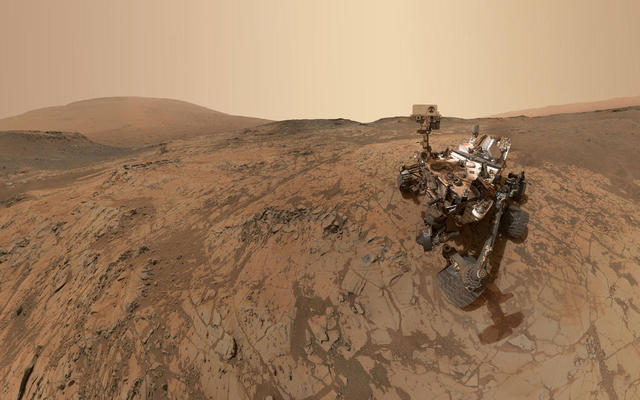
\includegraphics[width=\textwidth]{figures/Curiosity-Rover-Portrait-Mars-Mojave-Selfie-pia19142-MALHI-fi.jpg}
\end{figure}
  \begin{center}
    {\large
      Project Report%Insert document type (e.g., Project Report)
    }\\
    \vspace{0.2cm}
    {\Large
      B2-19%Insert your group name or real names here
    }
  \end{center}
  \vfill
  \begin{center}
  Aalborg University\\
  Robotics
  \end{center}
\end{titlepage}
\clearpage
\thispagestyle{empty}
{\small
\strut\vfill % push the content to the bottom of the page
\noindent Copyright \copyright{} Aalborg University 2017\par
\vspace{0.2cm}
%Copyright: group b2-19, robotics 
%\noindent Group B2-19 used sharelatex as a writing platform. %Furthermore the group met up in the group rooms everyday.
}
\clearpage
\pdfbookmark[0]{English title page}{label:titlepage_en}
\aautitlepage{%
  \englishprojectinfo{
    HADES - Interplanetary Exploration %title
  }{%
    Robotics theme
  }{%
    Fall Semester 2017 %project period
  }{%
    B2-19 % project group
  }{%
    %list of group members
    Anders Fischer Steen Jensen\\ 
    Violeta Kuldaite\\
    Natelia Mark\\
    Valdemar Jul Qvist\\
    Mark Richard Blankensteiner
  }{%
    %list of supervisors
   Jesper Abilgaard Larsen\\
    
  }{%
    1 % number of printed copies
  }{%
    \today % date of completion
  }%
}{%department and address
  \textbf{Robotics}\\
  Aalborg University\\
  \href{http://www.aau.dk}{http://www.aau.dk}
}{% the abstract
  This report aims to look into the basic necessities to manipulate a rover to autonomously explore and map an area on Mars, aswell as being able to be remote controlled.\\
The team has focused on looking into technologies that has been used on successful missions to Mars, to get an increased understanding of these technologies.\\
The main goal was to get the Turtlebot to function as if it was an exploration vehicle on Mars, but with severe limitations on the technology due to economical and time restraints.

}

%\cleardoublepage
%{\selectlanguage{danish}
%\pdfbookmark[0]{Danish title page}{label:titlepage_da}
%\aautitlepage{%
%  \danishprojectinfo{
%    Rapportens titel %title
%  }{%
%    Semestertema %theme
%  }{%
%    Efterårssemestret 2010 %project period
%  }{%
%    XXX % project group
%  }{%
%    %list of group members
%    Forfatter 1\\ 
%    Forfatter 2\\
%    Forfatter 3
%  }{%
%    %list of supervisors
%    Vejleder 1\\
%    Vejleder 2
%  }{%
%    1 % number of printed copies
%  }{%
%    \today % date of completion
%  }%
%}{%department and address
%  \textbf{Elektronik og IT}\\
%  Aalborg Universitet\\
%  \href{http://www.aau.dk}{http://www.aau.dk}
%}{% the abstract
%  Her er resuméet
%}}
\cleardoublepage
\pdfbookmark[0]{Contents}{label:contents}
\pagestyle{fancy} %enable headers and footers again
\tableofcontents
%\listoftodos
\chapter*{Preface\markboth{Preface}{Preface}}\label{ch:preface}
\addcontentsline{toc}{chapter}{Preface}
Here is the preface. You should put your signatures at the end of the preface.

\vspace{\baselineskip}\hfill Aalborg University, \today
\vfill\noindent
\begin{minipage}[b]{0.45\textwidth}
 \centering
 \rule{\textwidth}{0.5pt}\\
  Valdemar Jul Qvist\\
 {\footnotesize <vqvist17@student.auu.dk>}
\end{minipage}
\hfill
\begin{minipage}[b]{0.45\textwidth}
 \centering
 \rule{\textwidth}{0.5pt}\\
  Mark Richard Blankensteiner\\
 {\footnotesize <mblank16@student.aau.dk>}
\end{minipage}
\vspace{3\baselineskip}
\begin{center}
\begin{minipage}[b]{0.45\textwidth}
 \centering
 \rule{\textwidth}{0.5pt}
  Anders Fischer Steen Jensen\\
 {\footnotesize <afsj16@student.aau.dk>}\\
 \vspace{2 cm}
\end{minipage}
\end{center}
\begin{minipage}[b]{0.45\textwidth}
 \centering
 \rule{\textwidth}{0.5pt}\\
  Violeta Kuldaite\\
 {\footnotesize <vkulda17@student.aau.dk>}
\end{minipage}
\hfill
\begin{minipage}[b]{0.45\textwidth}
 \centering
 \rule{\textwidth}{0.5pt}\\
  Natalie Mark\\
 {\footnotesize <nmark15@student.aau.dk>}
\end{minipage}
\vspace{3\baselineskip}
\begin{center}
\begin{minipage}[b]{0.45\textwidth}
 \centering
 \rule{\textwidth}{0.5pt}
  Saman Rad\\
 {\footnotesize <srad15@student.aau.dk>}
\end{minipage}
\end{center}
\cleardoublepage
%mainmatter
\pagenumbering{arabic} %use arabic page numbering in the mainmatter
\chapter*{List of abbreviations\markboth{Listofabbreviations}{Listofabbreviations}} 
\label{ch:List of Abbreviations}

\begin{itemize}
    \item AC: Alternating Current
    \item AMCL: Adaptive Monte Carlo Localization
    \item C: Celsius
    \item CheMin: Chemistry \& Mineralogy instrument
    \item DC: Direct Current
    \item ECM: Electronically Commutated Motors
    \item fps: frames per second
    \item HazCam: Hazard Avoidance Cameras
    \item INEX: Interplanetary Exploration
    \item LIDAR: Light Detection And Ranging
    \item MOM: Mars Orbiter Mission
    \item MRO: Mars Reconnaissance Orbiter
    \item NASA: National Aeronautics and Space Administration
    \item NavCam: Navigation Cameras
    \item Pu-238: Plutonium-238
    \item px: Pixel
    \item RGB-D: Red, Green, Blue - Depth
    \item ROS: Robot Operating System
    \item SAM: Sample Analysis at Mars
    \item SLAM: Simultaneously Location And Mapping
\end{itemize}
\chapter{Introduction}\label{ch:introduction}

In 1965, after the first successful flyby mission to Mars by NASA, the interest in the planet mars increased considerably because they saw lots of similarities to earth \cite{NASAChronology}.\\
In 1996 NASA sent out a surface rover on the Pathfinder mission, which was the first successful rover to drive on Mars. The rover was named Sojourner, and it spent 85 days exploring the terrain, snapping photographs, taking chemical and atmospheric samples\cite{NASASojournerPathfinder}\cite{NASAChronology}.\\
In 2018 NASA will send out the lander InSight to investigate the deep interior of Mars. This will be done with modern technology to get a better understanding of the history of Mars and advance our knowledge about rocky planets\cite{InSight}.\\
%In 2020 NASA will be sending a rover to Mars for further investigation of bacterial lifeforms.%cite

The purpose of this project is to create a robot which can map the area, make a path and avoid obstacles on its own. Furthermore, the design of the robot has to be just as durable or more than the current solutions.\\


\begin{figure}[h]
    \centering
    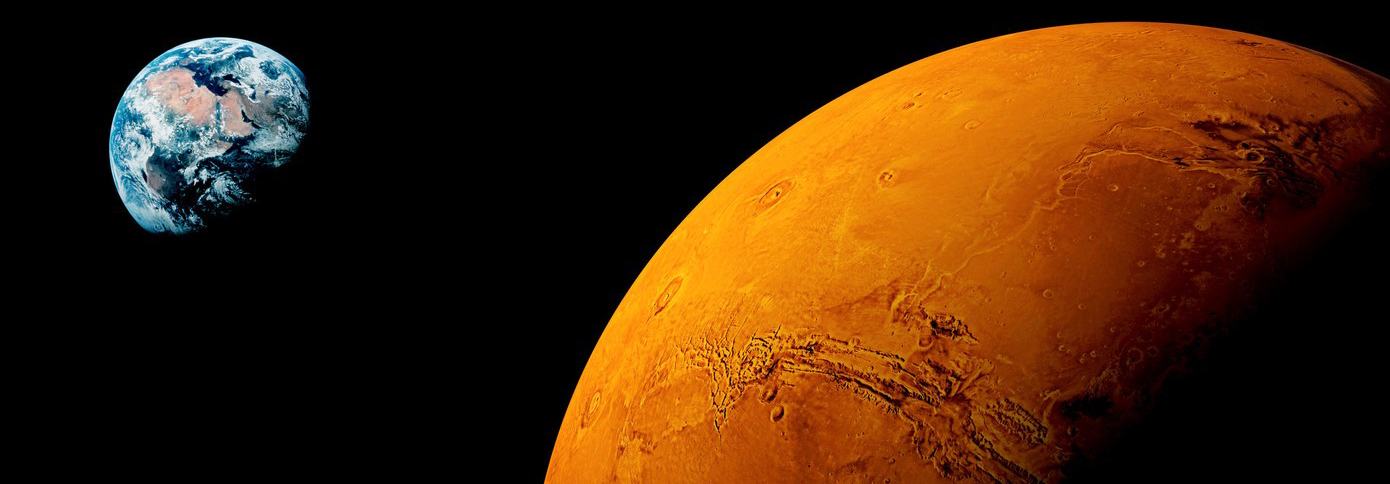
\includegraphics[width=\linewidth]{figures/639620382-mars.jpg}
    \caption{Picture of Mars and Earth\cite{MarsPics}}
    \label{fig:marsSeasons}
\end{figure}


\chapter{Initial problem statement}

The aim of this project is to design an autonomous robot, which can simulate an interplanetary rover on Mars. The robot has to drive in an unknown environment, while mapping the area and avoiding obstacles.\\ The robot has to have two types of controlling mechanisms, one which is automatic and one which is manual.\\
This project will look into the following:

[Maybe Main question] How to maneuver in an unknown environment
\begin{itemize}
\item How to map an area.
\item How to control the robot.
\item How to avoid obstacles.
%\item How to overcome delay time
%\item How to maneuver in an unknown environment
%\item How to communicate with INEX (satellites, etc.)
\end{itemize}



%link together this with the report






%To further the research on another planet we have been tasked to design an autonomous robot, which can scout and explore the surface of other planets.\todo{can we use "we" here?} How is it possible to explore new planets for humanity to inhabit. What will the requirements be for this interplanetary space-travel?\todo{Wait, do we want to know how to make the space-travel? Don't we just want to know how the robot can work on Mars?}

%\begin{itemize}
%\item How to map the area
%\item How do the robot avoid obstacles
%\item How to overcome the delay time (delay time of 14 min)
%\item How do we communicate with the robot (satellites, etc.)
%\item Control. (Left, Right, Forward and visual)
%\item How to maneuver in an unknown environment.
%\end{itemize}

%This report will look into the different components best suited for mapping and avoiding obstacles. Additionally, this report will contain an analysis of operational efficiency for INEX and a design description including the following components: Wheels, engine, fuel source, sensors, and other features. 
%\chapter{Approach}\label{ch:approachPerspective}
This chapter will provide an overview of how an approach to having a robot explore Mars and what future perceptive can be in exploring Mars, human colonization of Mars?


\section{Approach}
Talking about how to approach having a robotic explorer on Mars, it is needed to take in the many different variables when comparing Mars to Earth. Variables such as gravity, surface, radiation, weather, atmosphere, how much sunlight reaches Mars surface, and how the robot can navigate and map the area most efficiently. These parameters will help us determine the solution with chances of a working robot arriving on Mars and not breaking down due to unforeseen circumstances.\\
It is needed to know about the gravity as a factor, since it is very important that the robot can drive around in unknown environment, that is on Mars. It is therefore also important to know how the robots weight will impact its driving on Mars, since the gravity on Mars will make the robots weight seem different than on Earth.\\ 
The wheels for the robot will be chosen due to the surface on Mars, which is why it is important to consider how the soil on Mars will have a impact on the wheels. It is wanted that all wheels will remain on the surface to have traction and maneuverability. The surface will also have an impact on the way that suspension is designed and which kind of motor to use to make sure that the robot has a chance of moving.\\
The knowledge of the atmosphere on Mars, is of utmost importance, since the chemical composition will have influence on what material is going to be used for the robot. If the atmosphere is acidic, then the robot has to wear a non-corroding body, and the cables and wires must not dissolve and produce a short-circuit.\\ 
The atmosphere will have an impact on how much sunlight reaches the surface. This helps determine what kind of power source the robot should depend on. If enough sunlight shines through, the robot could run on solar panels, if not another option like Radioisotope Thermo-electric Generator could be used.\\
It is also important to know the radiation level on Mars. The robots may have to be radioactive hardened to sustain its mission, if there is a high level of alpha rays, beta rays and gamma rays on Mars, the robot may need to be shielded. Earth are protected by the core of Earth magnetic properties.
The robot will have different sensors attached to it, so it can examine the terrain and move around on Mars safely. What solution will be best suitable for the robot to have, will be determined beforehand, when it is known what Mars is like, and what is needed for the robot to move around, avoid obstacles and do the mapping and navigation of this\cite{WhatAreCosmicRays?}\cite{mmtg}.

%\section{Perspective}
%Is it possible for humans to live on Mars?
%When thinking the Earth might not last forever and the human survival instinct wants to find another solution as of living on another planet. There is still a lot of research needed to be done, before questions like these can be answered.
%Right now robots are patrolling the environment on Mars and exploring new territory, this will be described in more detail in chapter \ref{ch:existingSolutions}. 
%A robot, with the right components can patrol around on Mars with no risk to itself. It is not alive like humans and therefore does not need air to breathe or food to eat. As it is now, NASA have not yet discovered what ingredients there is in the water on Mars, and if it even is drinkable\cite{Curiosity2016}.


%Mars is only half the size of Earth, and there's only a part of the planet there's inhabitable, since the gravity is different all over the planet.\cite{howbigismars}\cite{gravity}
%As seen on figure \ref{fig:image003.jpg}, Earth and Mars are compared to each other as to the differences between the days in a year, gravity, sunlight and atmosphere.

%\begin{figure}[h]
%    \centering
%    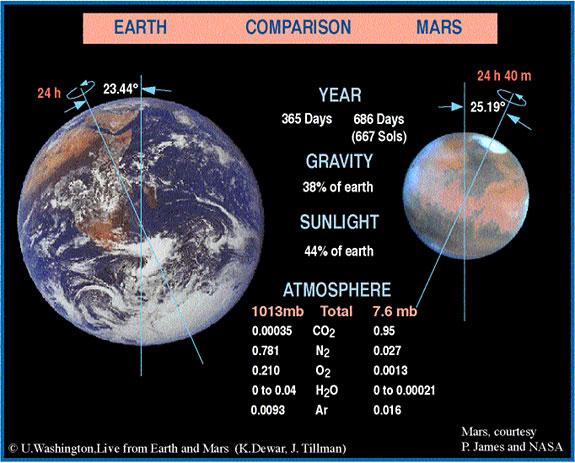
\includegraphics[width=.8\linewidth]{figures/image003.jpg}
%    \caption{Earth and Mars comparison \cite{gravity}}
%    \label{fig:image003.jpg} 
%\end{figure}



\chapter{Environment on Mars}\label{ch:environmentOnMars}

Mars, also called the Red Planet, was named by the Romans after the god of war because of its red, blood-like color, see figure\ref{fig:marsPicture01}. 

\section{Terrain} 
The martian terrain contains notable elements which are:

\subsection{Hellas Basin, and other craters}
Impact craters are remnants of past collisions with certain types of asteroid on the surface of mars. The craters vary in size, the largest is named Hellas basin which is 2253 kilometer in diameter and its floor is about 7,152 m  deep. The surrounding is a circular rim structure and look more like mountains with spaces between them.
the rim is 9,000 m higher than the bottom of the basin and the pressure at the bottom is 12.4  mbar which is  103 percent higher than the normal surface of mars  and because its above the triple point of water, liquid water could form in the basin under certain conditions. Hellas basin is thought to have formed about 4.1 to 3.8 billion years ago, during the period that large asteroids would hit Mars \cite{hellas}.

\subsection{Chaotic terrain}
On Mars there exist chaotic terrain, which is unlike anything we have on earth.\\
Chaotic terrain is terrain that has been created by old volcano flows having undermined the ground where it flowed, and then again at a later time ice will have covered the old flow,q but a new eruption has then created a new flow of lava which has run over the old flows, and thus created this strange terrain\cite{CTerrain}.

\subsection{Ice caps}
Seasonal Ice caps consist of carbon monoxide, water and dust, which covers both of Mars poles and can reach as high as 3 km in height and estimated to be as wide as 1000 km.

\subsection{Possible caves}
Observing from odyssey spacecraft, NASA scientists have identified seven possible caves. The entrance of these pits are 100 to 252 meters wide and they are believed to be around 70 to 96 meter in depth\cite{surface}\cite{guide}.

\subsection{Soil and water }
Mars surface is covered with rocks, sand and dust similar to some regions on earth. %except that no organic material has yet been found on mars.
The chemical composition of Mars soil can differ depending on where a sample has been taken, but the most known element found is iron in the form of rusting iron oxide, which gives the planet its famous red color.
\newline All evidence suggests that Mars used to have a watery past like that of earth, and water has been found in three states: solid ice, gas and occasionally liquid in some specific areas\cite{liquid}.
more than five million cubic kilometer of water in the form of ice  has been identified close to the surface of Mars\cite{water}.

\section{Climate of Mars}
The main composition of the martian atmosphere is carbon dioxide, and it has the surface pressure of 600 Pa where on earth, the atmospheric pressure on the surface is 101000 Pa.
\newline The surface of mars has a low thermal inertia, meaning that it heats up fast when under the sun light. At noon and near the equator, temperature reaches as high as 20$^{\circ}$C and at the poles it is around −153$^{\circ}$C. Thermal inertia changes in some areas on mars away from the poles, resulting in daily temperature swings and winds, which in return can pick up dust particles into the air and create clouds. Mars' atmosphere has a scale height of approximately 11 km\cite{climate}.
\begin{table} [h]
    \centering
    \begin{tabu} to 1\textwidth { | X[c] X[c] X[c] | }
     \hline
      & Earth & Mars \\ 
     %\hline
     %Average Distance from Sun & 150 million KM & 228.5 million KM \\  
     %\hline
     %Average Speed in Orbiting Sun & 29.7 KM/Sec & 23.3 KM/Sec \\
     %\hline
     %Diameter & 12,755.6 KM & 6,791.4 KM \\
     %\hline
     %Tilt of Axis & 23.5$^{\circ}$ & 25$^{\circ}$\\
     \hline
     Length of Year & 365.25 days & 687 Earth Days \\
     \hline
     Length of Day & 23 hours 56 minutes & 24 hours 37 minutes \\
     \hline
     Gravity & 9.82m/s$^2$ & 3.711m/s$^2$ \\
     \hline
     Temperature ranges from & -89$^{\circ}$C +55$^{\circ}$C &-153$^{\circ}$C at the poles +20$^{\circ}$C at equator \\
     \hline
     Atmosphere & Nitrogen, oxygen, & Mostly carbon dioxide, \\
      & argon, others & some water vapor \\
     %\hline
     %Number of moons & 1 & 2 \\
     \hline
    \end{tabu}
    \caption{Mars compared to Earth\cite{MarsVSEarth}}
    \label{tab:marsEarthFacts}
\end{table}

\newpage
\section{Safety on Mars}
To explore the Hellas Basin crater on Mars, these terrains has to be taken into consideration to prevent unnecessary damages to the robot, which could otherwise have been prevented.
One of the problems could be the chaotic terrain, where some places could be difficult to move over.\\
Another problem is that if the robot explores the northwestern rim of the crater, it could stumble upon the ice caps. The robot which has to avoid it, because there is no guarantee the robot to be clean for bacteria from earth, which is explained in chapter \ref{ch:Spacelaw}. In addition to this, The robot has to be able to detect all the definitions and respond appropriately \cite{AspectsWeather}.


%As mentioned earlier, Mars has four seasons due to the tilt of its rotational axis just like Earth. Mars’ orbit is slightly elliptical which affects the length of its seasons and is about 1.5 times farther from the sun than Earth’s orbit therefore the seasons on Mars lasts about twice as long, see figure \ref{fig:marsSeasons} for a graphic illustration of the difference between Mars and Earth when it comes to seasons\cite{MarsBasicFacts}\cite{MarsOverview}\cite{gravity}\cite{MarsInDepth}.


%As seen on figure \ref{fig:marsSeasons}, the months on Mars are not only longer than the ones on Earth, but the seasons’ positions are different as well. When there is summer and winter on Earth, Mars experiences autumn and spring. This has something to do with how the planets tilt of its rotational axis to do.\todo{rewrite.. A bit messy} Both Earth and Mars have close to the same axial tilt, but the two planets do not point in the same direction in space. This is the reason to why Mars is about one season ahead compared to Earth\cite{MarsSeasons}
.
%Make this table more beautiful later on: https://da.sharelatex.com/learn/Tables



%The average temperature of Mars is 77$^{\circ}$ Celsius colder than Earth, with an average temperature of - 63$^{\circ}$ Celsius, see table \ref{tab:marsEarthFacts}.

%In this figure \ref{fig:image003.jpg}, Earth and Mars are compared to each other as to the differences between the days in a year, gravity, sunlight and atmosphere. 

%\begin{figure}[h]
    %\centering
    %\includegraphics[width=.8\linewidth]{figures/im%age003.jpg}
    %\caption{Earth and Mars comparison %\cite{gravity}}
 %   \label{fig:image003.jpg} 
%\end{figure}



%https://mars.nasa.gov/allaboutmars/facts/#?c=inspace&s=distance

%Write about Radiation, atmosphere and sunlight
%It is important to know: atmosphere and how much sunlight reaches Mars surface






%https://www.nature.com/articles/ngeo2412






\chapter{Existing solutions}\label{ch:existingSolutions}

A set of different existing solutions exploring Mars, will be introduced in this chapter.

\section{Sojourner}\label{ch:existingSolutions_SojournerRover}
Sojourner was a six-wheeled rover that was the first to roam Mars.
Sojourner was built with a non-rechargeable battery that had a capacity of 150 Wh and solar cells with the size 0.22 \begin{math}m^2\end{math}, which could deliver around 15 W on the surface of Mars.\\ As communication Sojourner used a ultra high frequency radio modem, that talked to the lander, Pathfinder. Sojourner had three cameras on board with different lenses, two in front, which were monochrome and a color camera in the rear. Also a alpha proton x-ray spectrometer was implemented, it could tell the composition of the chemical elements present on the surface, but it could not detect hydrogen. Sojourner weighed 11.5 kg and were 65 cm in length. It had a mission length of 7 days, but it surpassed the mission and kept on working til day 85. Sojourner traveled over 100 meters in its 85 day long mission. It took 3 years to build, and had a cost of 175 million dollars\cite{Sojounerroverjpl}.

\section{Spirit and Opportunity} \label{ch:existingSolutions_SpiritOpportunity} 
The second generation of rovers that landed on mars were the two twin rovers. The mission of the two rovers was meant to last for at least 90 days, Spirit’s mission ended in 2014, but Opportunity's mission continued.\\ Opportunity has covered over 45 km on the surface of Mars. The rovers were meant to run 40 m in a day, or 1 cm per second. The wheels in the front and in the back could turn independently of each other, so the rover had a better turning ratio.\\
The rovers had two radioactive hardened CPU, one main, and one for backup. Furthermore, a 256 MB flash memory for storing pictures and data before it was sent back to Earth\cite{spiritopportunity_overview}.\\ They had nine cameras and six different scientific tools at disposal. One of the instruments was the panoramic camera that used two cameras with different color filters to detect structure and minerals. Another was the navigation tool, it used two monochrome cameras for navigation and driving, due to a wider field of view but with a lower resolution than the color cameras.\\The rovers kept themselves warm with a radioisotope heater that could generate 1 W of thermal energy.\\ For communication, the rovers had three different antennas, two for communicating with earth, and one for communication with the orbiter. The power was harvested from solar panels, which could recharge the batteries. These panels got covered by small dust particles but the weather on Mars creates small dust devils, that helps the rovers to be dust-free again\cite{Marsdust}.

\section{Curiosity}
\label{ch:existingSolutions_Curiosity}
Curiosity is the current rover on Mars. This vehicle was sent to Mars November 2011 and landed on Mars August 2012. Curiosity's sole purpose is to investigate the climate and geology of the Gale Crater\cite{CuriosityMissions}.\\ Curiosity is semi-autonomous and is intelligent enough to detect water and obstacles. One downside is that the satellites orbiting Mars only have the capacity to communicate with the rover sixteen hours a day due to the lack of orbiters communicating with Earth. When the scientists at NASA communicates with the rover it will take fourteen minutes for the signal to reach the rover\cite{CuriosityCommunication} \cite{CuriosityNASA}.\\
The rover found a water stream in 2016. NASA calculated that the rover itself might contaminate the stream, and since they couldn't sterilize Curiosity with a 100\% certainty, they were afraid of Earth bacteria would travel with the air and contaminate the whole water environment\cite{Curiosity2016}.\\
\newpage

\subsubsection{Instruments}

The thermal system of the rover is quite complex. The key components are covered in electrical heaters, and the heat and power is created by the isotope of plutonium-238.\\
Curiosity can drill into boulders and also vaporize samples to examine it's structure. When Curiosity drills, it will move the sample from the drill to either SAM or CheMin, which are built-in laboratories for the rover to handle evidence of environment.\\
In these bullet-points beneath you can read about the specific cameras NavCam and HazCam \cite{CuriosityNASA}\cite{CuriosityPOWER}: 

\begin{itemize}
\item Four Hazcams is mounted on the lower part of Curiosity. The HazCams use visible light to collect the data of the surroundings, they will then create a three-dimensional imagery of this data.\\ These cameras are created to help fine tune the movements for Curiosity in close proximity with hazardous obstacles. They work as the "eyes", but with a 120 degree vision for each of the four cameras. The 3-D imagery builds a map of the terrain with 3 meters and 4 as the farthest. It is mapping in triangular shapes, and placing the cameras in each direction this will make a square map for the AI to work in\cite{CuriosityVision}. 
\item The two pairs of NavCams is mounted on the mast of Curiosity. As the HazCams they use visible light to structure a 3-D map. They have a 45 degree field of vision, and the reason they are implemented is to correlate with the HazCams, and help structuring the imagery of the terrain \cite{CuriosityVision}. 
\end{itemize}



\section{Orbiters}
Orbiters is another way of exploring Mars. MRO is a satellite that takes close-up images of the surface and looks for mineral deposits. \\
A mission from India's space program, MOM, looks for different chemicals in the atmosphere such as \begin{math}CH$_4$\end{math} (methane). Methane has been detected by instruments on Earth, but has not been detected by Curiosity yet. If we detect methane on Mars then it means that Mars could have supported life.\\  Orbiters can be communication links from Mars to Earth and can also be used to transport lander-crafts such as rovers and probes\cite{orbitermro}.

\section{Stationary probes}
 Stationary probes can be used as a reconnaissance platform with tools. The probes can utilize robotic arms that dig into the ground taking soil samples. It also have cameras that can provide pictures of minerals and the landscape. Phoenix lander has a 2 meter high turret fitted with a stereo camera. These tools can provide knowledge of the environment for future missions.
The pathfinder lander probe also carried the first rover Sojourner to Mars\cite{Sojounerroverjpl} \cite{landerpho} \cite{landerpho1}.




%section what do they have in common? #wheels #cams etc
%\chapter{Economic aspects}
NASA scientist has published their budget in 2012 of \$18 billion, where more than 80\% of the budget was spent on robot programs and technology. The rest was spent on Cross-agency, IT, education and construction, environment, see figure \ref{fig:moneypiechartl}.
The budget covers a variety of expenses, including the rocket used to launch the spacecraft, and salaries for a team of highly skilled engineers, programmers, managers, scientists and independent contractors from around 20 states in the U.S, as well as Canada, Denmark and the U.K.\cite{EconomicNASA}.

\begin{figure}[h]
    \centering
    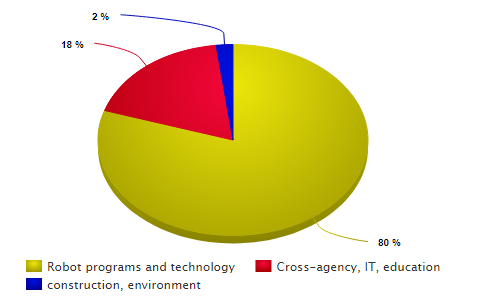
\includegraphics[[width=.8\textwidth]{figures/pieChart.png}
    \caption{NASA budget and distribution}
    \label{fig:moneypiechartl} %Make your own label so you can refer to it in the text. If you have trouble with this ask Natalie
\end{figure}

In addition to these achievements NASA is going to investigate more money on Mars rovers, exploring a deeper environment of Mars. This Project specifies a lot of time and money to send another more complicated robot to Mars.
Furthermore, Europe space agency (ESA) spend more than 5.77 billion dollars on the resources on Mars. But all preparations were unsuccessful. Despite bad projects, ESA is going to try to explore their resources in the future\cite{EconomicESA2}\cite{EconomicESA}.

\chapter{Space Law} \label{ch:Spacelaw}
Space Law is the description of the laws governing all space-related activities.
Space Law comprises a variety of international agreements, treaties, conventions, United Nations resolutions as well as rules and regulations of international organizations. The main body of the Space Law is commonly named the “Five United Nations treaties on outer space”, which have all been signed by the three depository governments: the Russian Federation, the United Kingdom and the United States of America.

\section{The “Outer Space Treaty”}
This treaty is the main source which other treaties derive from. It covers the principles regarding exploration and use of outer space, which includes the Moon, and other celestial bodies.\\
Below is stated six articles related to driving a robot on Mars:

\subsection{The “Rescue Agreement”}
This treaty is focusing on the agreements about rescuing Astronauts, as well as returning objects launched into outer space.\\
The agreement elaborates on Article 8[appendix Articles] of the “Outer Space Treaty”, which provides that states shall take all possible steps to rescue and assist astronauts in distress, and upon requests provide assistance in recovering space objects which has returned to earth outside the territory of the launching state\cite{Treaty2}.

\subsection{The “Liability Convention”}
This treaty is an elaboration to article 7 of the “Outer Space Treaty” which states:
“Each State Party to the Treaty that launches or procures the launching of an object into outer space, including the moon and other celestial bodies, and each State Party from whose territory or facility an object is launched, is internationally liable for damage to another State Party to the Treaty or to its natural or juridical persons by such object or its component parts on the Earth, in air or in outer space, including the moon and other celestial bodies\cite{Treaty3}.”

\subsection{The “Registration Convention”}
This treaty is built upon the desire for a mechanism which can assist in identifying space objects, which has then since 1962 been upheld by the United Nations, to keep an open registry of any space object. 
To this date 92 percent of all satellites, probes, landers, manned spacecraft and space station flight elements launched into earth orbit or beyond have been registered with the Secretary-General of the United Nations\cite{Treaty4}. 

\subsection{The “Moon Agreement”} \label{ch:moonAgreement}
This Agreement reaffirms and elaborates on many of the provisions of the Outer Space Treaty as applied to the Moon and other celestial bodies, providing that those bodies should be used exclusively for peaceful purposes, that their environments should not be disrupted, that the United Nations should be informed of the location and purpose of any station established on those bodies. In addition, the Agreement provides that the Moon and its natural resources are the common heritage of mankind and that an international regime should be established to govern the exploitation of such resources when such exploitation is about to become feasible\cite{Treaty5}.

\subsection{Conclusion}
These laws are especially important to this project, for the reason that it establishes some rules for what we need to avoid, as in the "Moon Agreement" we talk about not contaminating or disrupting the environment, which is one of the core reasons why the robot should avoid areas with water.\\
The "Liability Convention" is also really important, since it helps clarifying who is to be liable in case our robot breaks other governments equipment, or contaminate an area with micro bacteria.

\chapter{Safety}

To explore Mars it is necessary to take the safety of the robot into account. The Martian environment has to be taken into consideration, to keep the robot safe.
As described in chapter \ref{ch:environmentOnMars} the temperature ranges differs a lot, which is why a robot on Mars needs to be able to handle such range of temperatures. Additionally, it is also important to take into consideration, that there are dust storms on Mars, see figure \ref{fig:Duststorm }. The strongest wind during dust storms is 97 km/h. A robot in this environment has to have a low center of mass to handle these strong winds\cite{AspectsWeather} \cite{AspectsTemperature}.

\begin{figure}[h]
    \centering
    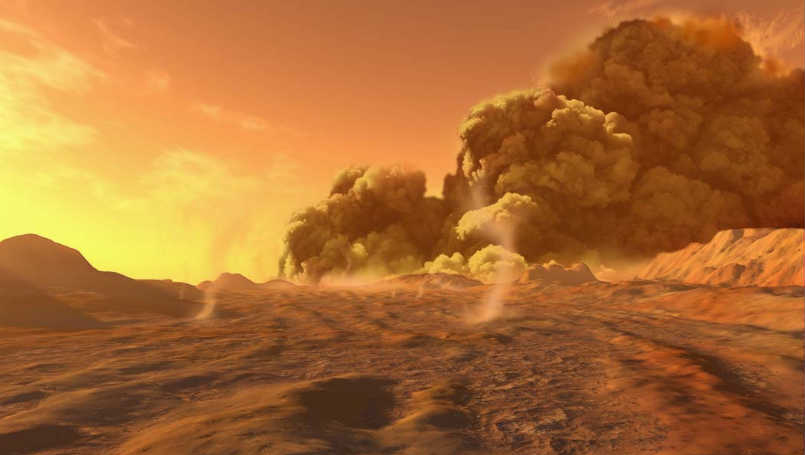
\includegraphics[width=.7\textwidth]{figures/dust-storm-on-mars2.jpg}
    \caption{Artist impression of dust storm on Mars \cite{Duststorm}} 
    \label{fig:Duststorm } 
\end{figure}

For the safety of the Martian environment, a robot on Mars has to keep its distance to water, ice, and other geology definitions due to specific regulations, as explained in chapter \ref{ch:Spacelaw}. In addition to this, INEX has to be able to detect all the definitions and respond appropriately\cite{AspectsWeather}.


%The atmosphere of Mars consists of 95\% CO$_2$. During the winter, the atmosphere is cold enough to condense CO$_2$ into CO$_2$-ice caps.

%extra

%\newpage

%\section{Social Aspects}
%\begin{figure}[h]
    %\centering
    %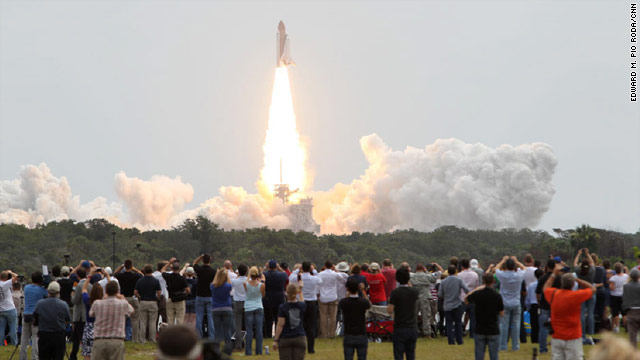
\includegraphics[width=\textwidth]{figures/1356.jpg}
    %\caption{ALWAYS REMEMBER CAPTION UNDER PICTURES (edit the label and a picture if there is a %picture you HAVE to refer to it in the text, which you do with the label) AND remember cite %if it's not your own picture/illustration}
    %\label{fig:randomfiglabel} %Make your own label so you can refer to it in the text. If you have trouble with this ask Natalie
%\end{figure}%\todo{Caption and label in picture needed}

%Nowadays any technological progress that is able to make it to the mainstream media
%has a strong impact on the general thinking of society.
%Exploring space and being able to go beyond Earth's orbit, has been one of the goals that has formed modern mentality of human society in a way that once, being able to fly did.
%Each question we find the answer for, becomes a doorway for more questions and creates the ground for means of answering them.
%The one planet that attracts the most attention and curiosity, is our closest neighbor Mars.
%Raising the chances for a project to get funded goes hand in hand with how much influence it can create on the targeted area and that's the fact.\\
%Considering the Mars missions and the changes in perspectives our new understandings of this planet could bring about, we could always expect positive social reinforcement and look at society as one of the main sources of feedback.%\todo( find or add some source )
\\



\chapter{Technical Proposal}\label{ch:solutionProposal}
This chapter will propose different types of sensors, wheel systems and energy sources, general materials and software.

\section{Sensors}
INEX will need a sensor to scan its surrounding area for mapping and obstacle avoidance.

\subsection{Laser}
An autonomous vehicle will need to alter its path when objects occur. One of the most efficient ways for the vehicle to follow a trajectory is with structured light.\\This light will project a triangular image for the image sensor processor to process. It will then derive the range and bearing for the illuminated object from the beam of structured light and match it to the current position of the vehicle\cite{Lasers}.


\subsection{Radar}
Radars use a highly concentrated radio wave, if there's any obstacles on its way, it will reflect electromagnetic energy. The sensor will then pick up the signalling energy and measure the time spent on getting the "echo" back\cite{Radar}.

The further away the transmission has to be sent, the lower the frequency has to.
Satellites are typically using C-band ( 300 MHz - 1 GHz ). 
For avoidance on the other hand, it will be of utmost importance for us to get higher frequencies, since the system has to maneuver at high accuracy. This frequency for avoidance will generalized be at I- or J-band (8-12 GHz)\cite{RadarTutorial}.

%\begin{figure}[h]
    %\centering
   % 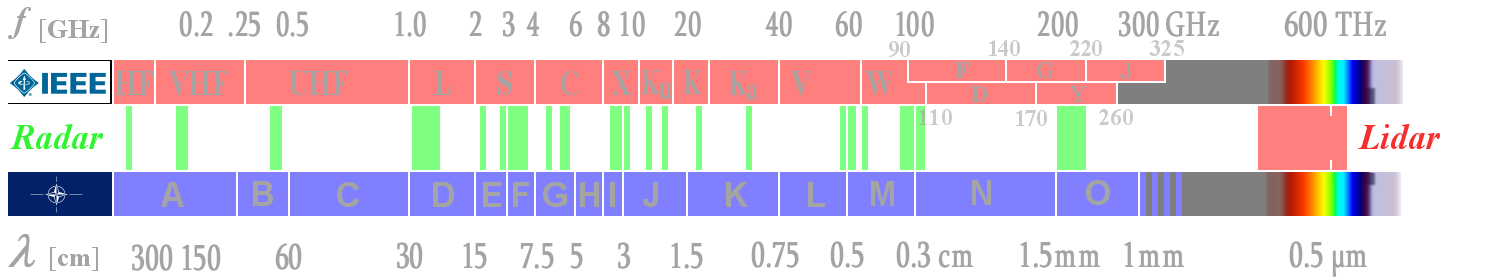
\includegraphics[width=\textwidth]{figures/radarfrequencies.png}
  %  \caption{Radar Frequencies \cite{RadarTutorial}}
 %   \label{fig:radarfrequencies.png}
%\end{figure}


\subsection{LIDAR}
Since the most common platforms for LIDAR is airplanes, this remote-sense and GPS uses the light from the surface of earth to reflect and then scan the surroundings. This method is used for both its accuracy and differentiating man-made versus nature structures\cite{LIDAR}.

\subsection{Cameras (RGB-D)} \label{ch:CameraRGB}

Some RGB-D uses a night-vision camera and a laser that produce a unique cloud of points. The camera triangulates the distance to the different points from the laser. This triangulation can then be translated into map with depth, that will let the robot determine the distance to different objects. 
A downside to the night vision RGB-D cameras is that it does not work in sunlight. This is because the infrared light rays interferes with the camera\cite{Cameras}.

\subsection{Ultrasonic sensors}
Ultrasonic sensors uses sound waves to measure distance to various obstacles. One part of the sensor called a transducer, emits a sound wave that hits the surface, bounces back and gets picked up by the receiver. 
%To calculate how far away a set of objects is, the wave formula is needed to calculate the velocity of the wave. Lambda is the wavelength, f is the frequency of the wave and v is the velocity.
%\begin{equation}\label{eq:ultrasonic01}
 %   v= \lambda \cdot f
%\end{equation}
%For calculating distance(d) back and forwards the velocity is needed and the time (t) for the signal to be sent and received. 
%\begin{equation}\label{eq:unltrasonic02}
 %  d=t\cdot v 
%\end{equation}
%The distance has to be halved, because the time is from the transducer to the receiver.
%\begin{equation}\label{eq:unltrasonic03}
 %  DTO=d/2
%\end{equation}
Ultrasonic sensors is a cheap solution, but sound can deflect different from some surfaces, which is a problem. They can also be sensitive to noise in the signal and the sensor does not have a good sense of direction because of the sound wave is fan-like shaped. All this can be overcome by using an array of ultrasonic sensors to help build up a more accurate map, by having multiple inputs from the array\cite{Ultrasonicsnesor}.
%\newpage
\section{Motors}
An electric motor converts electrical power into mechanical rotation, that can turn the Wheels of HADES.
In this section will propose two different possible types of motors HADES could end up using.

\subsection{AC motor}
AC motors consist of two main part. A stator and a rotor. The stator is a stationary part and the rotor is a rotating part. The rotor is located inside of the stator and due to magnetic fields inside of the stator, the rotor will rotate\cite{motor21}.\\ 
AC motor use a alternating current see figure \ref{fig:ACmotor}. Due to the slip-rings, the AC motor provides energy to the robot\cite{motor21}.

\begin{figure}[h]
    \centering
    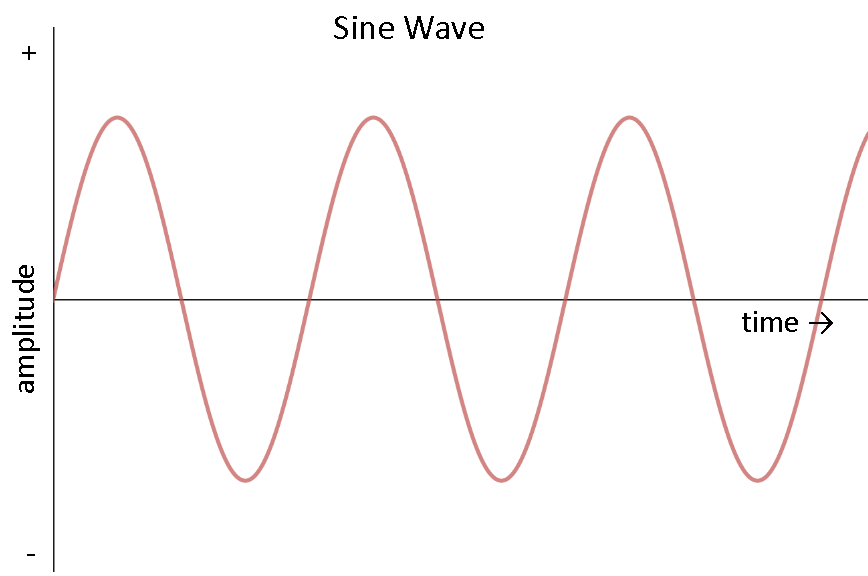
\includegraphics[width=.6\linewidth]{figures/wave.png}
    \caption{Alternative current\cite{ACmotor3}}
    \label{fig:ACmotor}
\end{figure}

\subsection{Brushless DC motor}
The working process of a brushless DC motor is similar to an AC motor. The main difference between a brushless DC motor and an AC motor is how they produce energy. Furthermore, brushless DC motors use commutator instead of slip rings to create a current energy.\\ 
The brushless DC motor have around 85\%-90\% efficiency.The advantage of brushless DC motor is less noisy\ref{fig:DCmotor}\cite{DCbrusshles}.

\begin{figure}[h]
    \centering    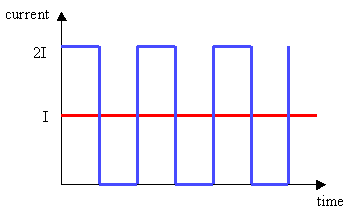
\includegraphics[width=.6\linewidth]{figures/dcMotor.png}
    \caption{Brushless DC curve angular\cite{Graphdd}}
    \label{fig:DCmotor}
\end{figure}

 %\newpage

\subsection{Conclusion} 
Brushless DC motors is more advance and controlling system are more simple than AC motor. In addition to this, HADES using brushless DC motor will be controlled easier.

\section{Wheel systems}
The robot will need to be able to move around and therefore wheels or continuous tracks are needed. This part will describe the advantages and disadvantages of the two different types of wheel systems.


\subsection{Wheels}\label{ch:Wheels}
%\textbf{Advantages}\\
Wheels have several advantages in comparison to track systems. One of the most relevant advantages is the weight of the wheels, since they can be made in many types of materials, without losing to much durability.
Another advantage is the low production costs, and simplicity of wheel types, since they do not have too many complex moving parts. This makes them cheaper to manufacture. Because there are few moving parts, there is a chance that sand and dust from the surface of Mars will get stuck in places that will decrease the mobility. 
Being able to control the wheels individually will increase the maneuverability.

%\textbf{Disadvantages:}\\
Wheel types have a few disadvantages. One of these is when the robot has to climb over rocky terrains, it would not be able to get across vertical obstacles with at least half the height as the diameter of the wheels. On slippery surfaces, wheels will have a harder time to get a strong grip and the robot can end up getting stuck in place, or having to consume more energy to move\cite{Wheels1}\cite{Wheels2}.
%could be
\subsection{Continuous Tracks}
%\textbf{Advantages}\\
The advantages of track systems, is that they have a high power delivery efficiency, which is optimized to a high performance when going through rough terrains.
Using tracks also allows for heavy loads, because the weight is getting spread to the entire surface of the tracks, compared to wheels, the weight is only being distributed to where the wheels make contact with the ground.

%\textbf{Disadvantages}\\
On the other hand, tracks have a more complex mechanical system compared to wheel systems, which means they can break down more easily compared with wheels, if sand stone or dust gets stuck somewhere, which requires a higher degree of maintenance if it should not break down.
Another issue with track systems is that they are less precise in maneuverability, since their movements are all based on 2 points of contact to the ground. This contact spans over a larger area than wheels and for this reason it also required more power to make turning movements with track systems\cite{Wheels1}\cite{Wheels2}.

\section{Energy source}

In space exploration there exists two sources used for generating power to the space vehicles. One is solar power and the other one is a warm decaying isotope. \newline This part will describe those two types of energy sources.

\subsection{Solar power}

Solar power is produced by solar cells. A solar cell is made of layers of silicon stacked on each other, one layer with a positive charged atoms and other layers is of negative charged atoms. A silicon crystal holds the atoms in a grid shape. When the photons hits the surface of the cell, the photon kicks one electron from the grid on the negative charged side. Then it moves through a wire to the positive charged side, this is where the power is created. When electricity is produced it has to be used or stored in a battery, so it can be saved and used when more power is needed, for example when there is no sun available.\cite{SolarPanels}.\\

\textit{"Most solar panels used in home solar arrays come with a warranty for some 25 or 30 years"}\cite{SolarPanels}
The solar panels do not wear out easily, meaning it will keep on being a useful energy source for decades.




\subsection{Radioisotope thermoelectric generator}

This method relies on a heating source, which comes from a decaying isotope of plutonium called Pu-238. For converting heat to electricity it uses a method called thermocoupling. Thermocoupling works by having two different metals attached to each other at one end and heating up that end, this will produce a small current.
A radioisotope thermometric generator has an efficiency around 6 to 7\% the rest is still heat and can be used to keep the core of the robot and it's tools warm. The radioisotope thermometric generator method has been used in many space missions and is a very reliable source of energy\cite{RTG}.



\section{Materials}
Material used in space missions, must be light enough, and have the ability to withstand the harsh environment of the space.
The ability to manipulate different parts of the rover and repair them if needed during the mission is highly limited due to different reasons, such as the communication delay and the complexity of a comprehensive repair mechanism. This results in the reliability of materials that sometimes are difficult to contain or attain. A good example to this would be the radioisotope of certain elements used in thermo-electric batteries which are extremely complicated to handle yet more reliable than solar panels\cite{NuclearPower}. \\ Due to the radiation level inside the robot coated electrical components is needed, so that it is not effected by the radiations.\\
 Different kind of material would be used to explore caves or inaccessible areas on earth. Considering that, erosion could have different meanings on mars compared to earth.


\section{Conclusion}
To avoid obstacles, a robot needs a camera to percieve the surroundings. The LIDAR sensor, with a 360$^{\circ}$ field of vision and looking up to 120 m into the distance, is a useful feature for scanning the surroundings and detecting obstacles.\\
As for the moving part, either wheels or continuous tracks can be used as a solution. Both types have advantages and disadvantages. Wheels are faster, more precise in maneuverability but are more complex in its construction than continuous tracks.\\
The energy source solar power is dependent on sunlight, which means sun is needed in this process for generating power. The RTG method can work in any environment, meaning that it does not depend on sunlight. It is mentioned earlier than Pu-238 is a reliable source of energy, where solar panels wear out after years.


\input{sections/problemAnalysis/SolutionProposal/SLAM.tex}
\chapter{Solution Description}\label{ch:solutionDescription}

 

This chapter will introduce and describe the different elements chosen for the final design. Furthermore it will be explained why these parts have been chosen compared to the other possible components.

\section{Final problem formulation}\label{ch:finalproblem}
%How is it possible to design an autonomous vehicle that can move around in an unknown area. While the vehicle has to autonomously navigate and avoid obstacles.
%How can a robot be designed so that it can map, move in an unknown area and avoid obstacles? 
%How is it possible to design a rover that can move in an unknown area while map and avoid obstacles?
%How is it possible to design a rover that uses SLAM for moving in an unknown area while mapping and avoiding obstacles?
%It is possible to create a robot with existing solutions, who? can avoid obtacles and map the area by his own in unknown places?

How is it possible to design a rover that uses SLAM for automatically moving in an unknown area while mapping and avoiding obstacles, but also possible to be controlled manually.



\section{Design delimitation}\label{ch:Designdelimitations}

Below is stated delimitations for the solution proposal:

\begin{itemize}
    \item The robot has to operate in an unknown outdoor area.
    \item The robot has to stay clear of obstacles with a height of more than 5 cm. 
    \item The robot has to be able to climb a grading of 7\% without getting stuck.
    \item If an obstacle is not avoidable the robots has to call for human interaction.
    \item The robot may not move more than 5 meters pr 14 minutes due to time delay.
\end{itemize}

\section{Design Requirement Specifications} \label{ch:Designrequiremnts}

The robot is required to have enough space to fit scientific tools inside the base.\\  
The distance between ground and chassis should be at least 50 cm and the width of the robot should be the same as an average car.\\ 
The robot needs a field of vision of at least 10 meters, since the hazards of sink holes and cliffs should be present.\\
The maximum velocity of the robot should be 0,006 m/s so the operators have a chance to stop the robot interfering with hazardous areas.\\
The camera will need a 360 degree of view implemented under the base. A way to apprehend damages to the camera by the environment, the camera will be surrounded with acrylic panzer glass \todo{source for self-repairing glass}\cite{Lidar360}.\\ 
The robots internal has to be protected from radiation, since radiation can be more or less damaging to different materials\cite{radiationEffectsInMaterials}.\\
The robot needs a redundant circuit of electronics, such as if the system breaks down a backup system can still operate the robot.\\
The wheels of the robot needs to have a high friction due to the sand surface on Mars\cite{sand}.

\section{Design proposal}\label{ch:Designproposal}
This section will give a short description of how the robot should function.\\
The robot needs motors to accelerate, decelerate and overcoming the incline that is set at a maximum of 7\%. For vision the robot will use a LIDAR sensor for detecting and ranging the terrain.\\
For the robot to move through the perceived environment, it will need a algorithm to assist moving autonomously.\\

\chapter{Implementation theory}

\section{Software}

\subsection{Rviz} \label{ch:Frontier Exploration}

\subsection{Mapping}

\subsection{Localization}

\subsection{SLAM}

SLAM is not a specific algorithm, but a concept where there are many different approaches. SLAM uses a collection of data gathered from varies sensors such as odometry and distance measuring sensors, to build a map and to know where it is located in the map.
There are different solutions to SLAM some are made for indoor use others for outdoor, underwater, and some is made to navigate in an area with terrain. Odometry is a measurement of how much the wheels have rotated. This can be unreliable due to wheels are slipping or other reasons. Furthermore, this "noise" in the signal can be dealt with using it in combination of odometry and a gyroscope that measures the rotation and movement in different directions.\\
When the robot starts mapping it looks with its sensors, such as cameras, LIDAR, laser, etc. for objects. After, the robot moves forward, measures how far it moved with the odometry sensor and gyroscope, then looks at on the surrounding area to see new relation with objects\cite{SLAMdummies}\cite{DifferentSLAM}\cite{GyrosOdometry}.\\
A simple algorithm for SLAM could be:
\begin{itemize}
    \item Scan area for objects
    \item Move forward and measure how far
    \item Scan again for objects
    \item Look for reappearing objects
    \item Triangulate location to objects that reappeared
    \item Relocate the robot in the map 
\end{itemize}

\subsection{Algorithm for avoid obstacle}



\chapther{Implementation Theory}\label{ch:Implementationtheory}

\section{Turtlebot} %chassis

\section{Computer} 
The computer is an ASUS notebook, it has an Intel core i3-4010U CPU that has 2 cores and operate at 1.7MHz\cite{CPU}. The notebook has 4GB RAM and an integrated HD graphics card on the motherboard\cite{ASUS}.
The operating system is Ubuntu 16.04 LTS a layer for the Linux distribution. For communication between the sensors and the Turtlebot, the computer uses USB 2.0.

\section{Sensor}

\section{Code}
\section{Life span}
The %Life is short, but coffee fixes everything #YOLO
\chapter{Communication}
\chapter{Conclusion}\label{ch:conclusion}
In case you have questions, comments, suggestions or have found a bug, please do not hesitate to contact me. You can find my contact details below.
  \begin{center}
    Jesper Kjær Nielsen\\
    \href{mailto: jkn@es.aau.dk}{jkn@es.aau.dk}\\
    \href{http://kom.aau.dk/~jkn}{http://kom.aau.dk/\textasciitilde jkn}\\
    Fredrik Bajers Vej 7\\
    9220 Aalborg Ø
  \end{center}
\printbibliography[heading=bibintoc]
\label{bib:mybiblio}
\appendix
\end{document}